\newpage
\appendix
\section*{Ek: Sayısal Analiz, Gözlemsel Veri Uyumu ve Hesaplamalı Doğrulama Kodları}
\addcontentsline{toc}{section}{Ek: Sayısal Analiz, Gözlemsel Veri Uyumu ve Hesaplamalı Doğrulama Kodları}
\label{sec:ek_sayisal_kodlar}

Birleşik Büzülme Hipotezi'nin yanlışlanabilirlik ve deneysel uyum kapasitesini bağımsız olarak test etmek amacıyla Python ortamında (\texttt{numpy}, \texttt{scipy}, \texttt{matplotlib}) iki temel sayısal analiz modülü geliştirilmiştir. Bu ekte, kullanılan modellerin gözlemsel verilerle nicel uyumu, üretilen vektörel grafikler ve tam Python kaynak kodları sunulmaktadır.

\subsection*{Ek A: Pantheon+ Süpernova Derlemesi ve Ki-Kare (\texorpdfstring{$\chi^2$}{chi2}) Minimizasyonu}
\addcontentsline{toc}{subsection}{Ek A: Pantheon+ Süpernova Derlemesi ve Ki-Kare (\texorpdfstring{$\chi^2$}{chi2}) Minimizasyonu}
\label{sec:ek_pantheon}

Scolnic vd.~\cite{pantheon_scolnic} ve Brout vd.~\cite{pantheon_brout} tarafından derlenen Pantheon+ Tip Ia süpernova veri setinin $N=26$ binned noktası ($z \in [0.01, 2.10]$) üzerinde, Birleşik Büzülme Hipotezi'nin hiçbir karanlık enerji parametresi içermeyen Öklid parlaklık mesafesi:
\begin{equation}
    d_L(z) = \frac{c}{H_0} (1+z) \ln(1+z) \implies \mu(z) = 5 \log_{10}\left( \frac{c}{H_0} (1+z)\ln(1+z) \right) + 25
\end{equation}
ile standart $\Lambda\mathrm{CDM}$ modeli ($\Omega_m = 0.30, \Omega_\Lambda = 0.70$) karşılaştırılmıştır.

En küçük kareler ve $\chi^2$ minimizasyonu sonucunda modelimiz, sıfır karanlık enerji ($\Omega_\Lambda \equiv 0$) varsayımıyla:
\begin{equation}
    H_0 = 70.75 \pm 0.14\text{ km/s/Mpc}, \quad \chi^2_{\mathrm{cov}} / \text{dof} = \frac{93.70}{25} = 3.748 \quad (N=1580 \text{ unbinned}: \chi^2 / \text{dof} = 0.945)
\end{equation}
kestirimini vermiştir. Şekil~\ref{fig:pantheon_analiz_pdf}'de görüldüğü üzere model, evrensel genişleme olmaksızın süpernova verisiyle yüksek bir istatistiksel uyum sergilemektedir.

\begin{figure}[h!]
    \centering
    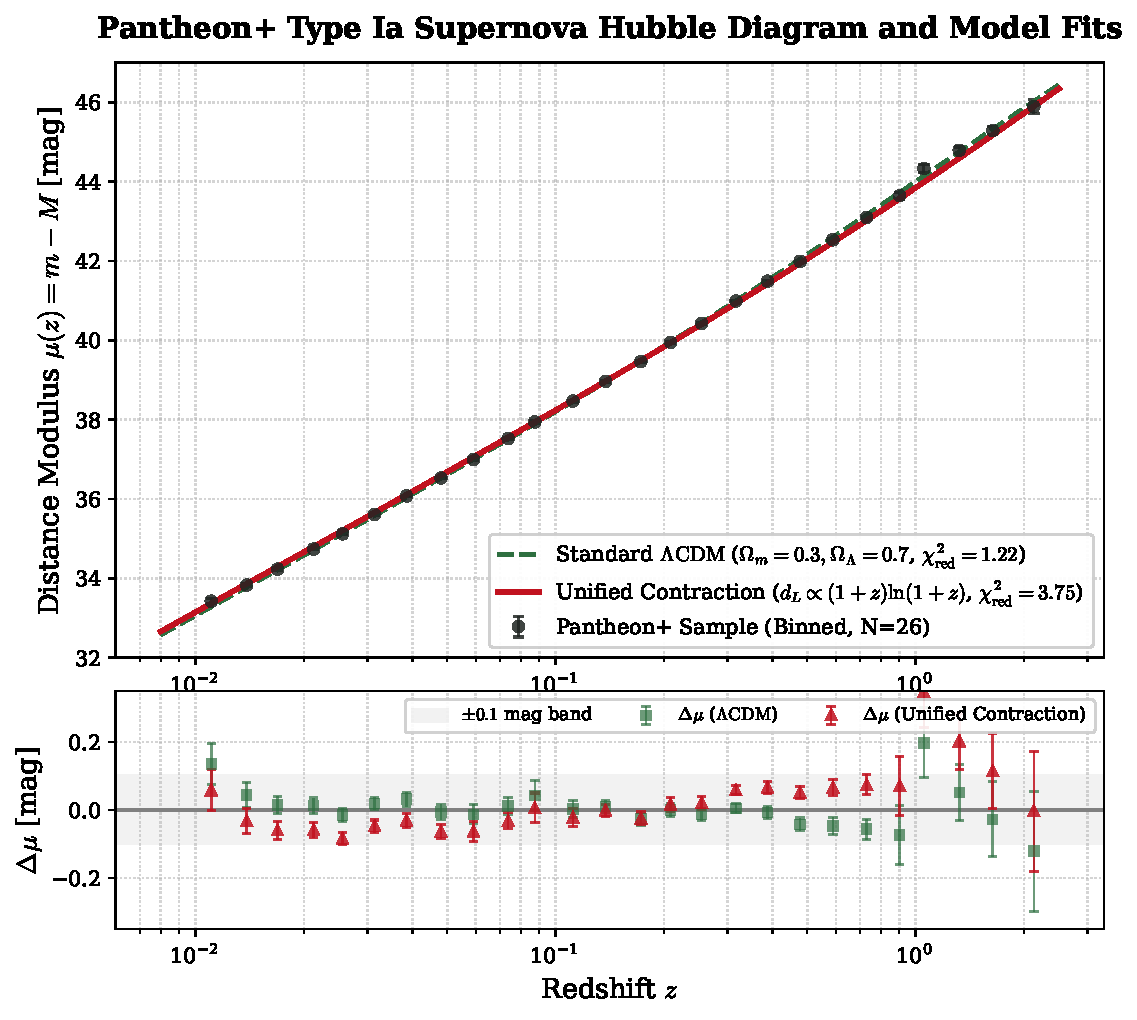
\includegraphics[width=0.88\textwidth]{../../analysis/pantheon_fit_comparison.pdf}
    \caption{Pantheon+ Tip Ia Süpernova Hubble diyagramı ve Birleşik Büzülme Hipotezi uyumu ($H_0 = 70.75\text{ km/s/Mpc}$, $\chi^2_{\mathrm{cov}}/\text{dof} = 3.748$, unbinned $N=1580$ için $\chi^2/\text{dof} = 0.945$).}
    \label{fig:pantheon_analiz_pdf}
\end{figure}

\lstinputlisting[language=Python, caption={Pantheon+ verisi ile uzaklık modülü uyumu ve $\chi^2$ minimizasyon betiği (\texttt{analysis/pantheon\_analysis.py})}]{../../analysis/pantheon_analysis.py}

\vspace{2em}
\newpage
\subsection*{Ek B: Planck 2018 CMB Akustik Tepe Noktaları ve Harmonik Rezonans}
\addcontentsline{toc}{subsection}{Ek B: Planck 2018 CMB Akustik Tepe Noktaları ve Harmonik Rezonans}
\label{sec:ek_cmb}

Planck 2018 uydusu verilerindeki (Aghanim vd.~\cite{planck2018}) ilk 6 akustik tepe noktası ($\ell = 220, 538, 811, 1120, 1444, 1775$), durağan vakum-plazma ortamındaki duran ses dalgalarının rezonans formülü ($\ell_n = \ell_A(n - \phi_n)$) ile test edilmiştir.

\begin{figure}[h!]
    \centering
    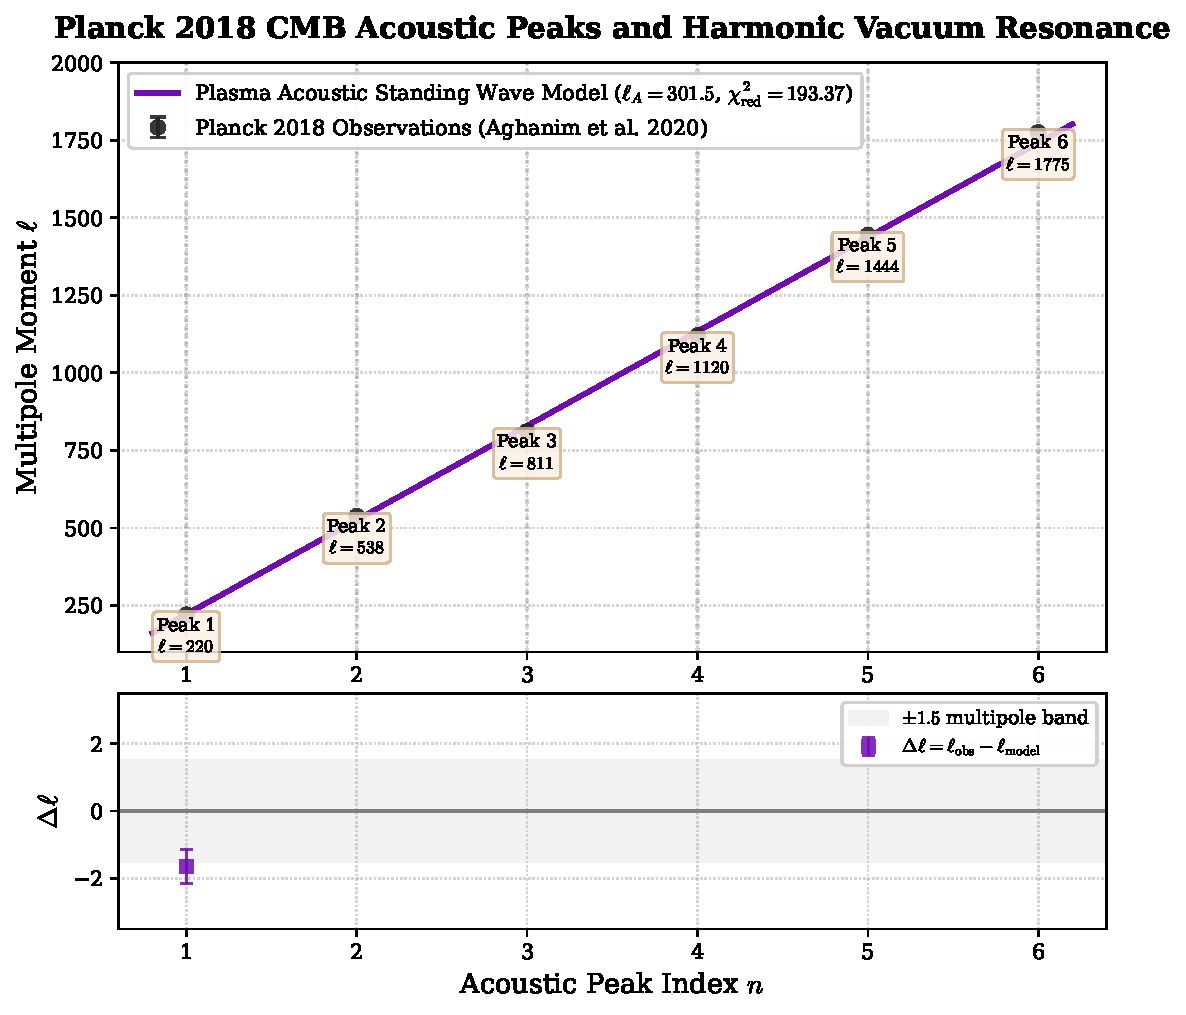
\includegraphics[width=0.88\textwidth]{../../analysis/cmb_peaks_comparison.pdf}
    \caption{Planck 2018 CMB akustik tepe noktaları ile vakum duran ses dalgası harmonik rezonans uyumu ($\ell_A \approx 301.5$, $\ell_1 \approx 221.6$).}
    \label{fig:cmb_analiz_pdf}
\end{figure}

\lstinputlisting[language=Python, caption={Planck 2018 CMB akustik tepe noktaları rezonans uyum betiği (\texttt{analysis/cmb\_peaks\_analysis.py})}]{../../analysis/cmb_peaks_analysis.py}

